\documentclass[margin=1mm]{standalone}

\usepackage[x11names]{xcolor}
\usepackage{tikz}
\colorlet{fascist}{OrangeRed1}
\colorlet{liberal}{Turquoise4}
\usepackage{graphicx}
\usepackage{fontspec}
\setmainfont{QTHeidelbergType}
\usetikzlibrary{patterns}

\begin{document}
	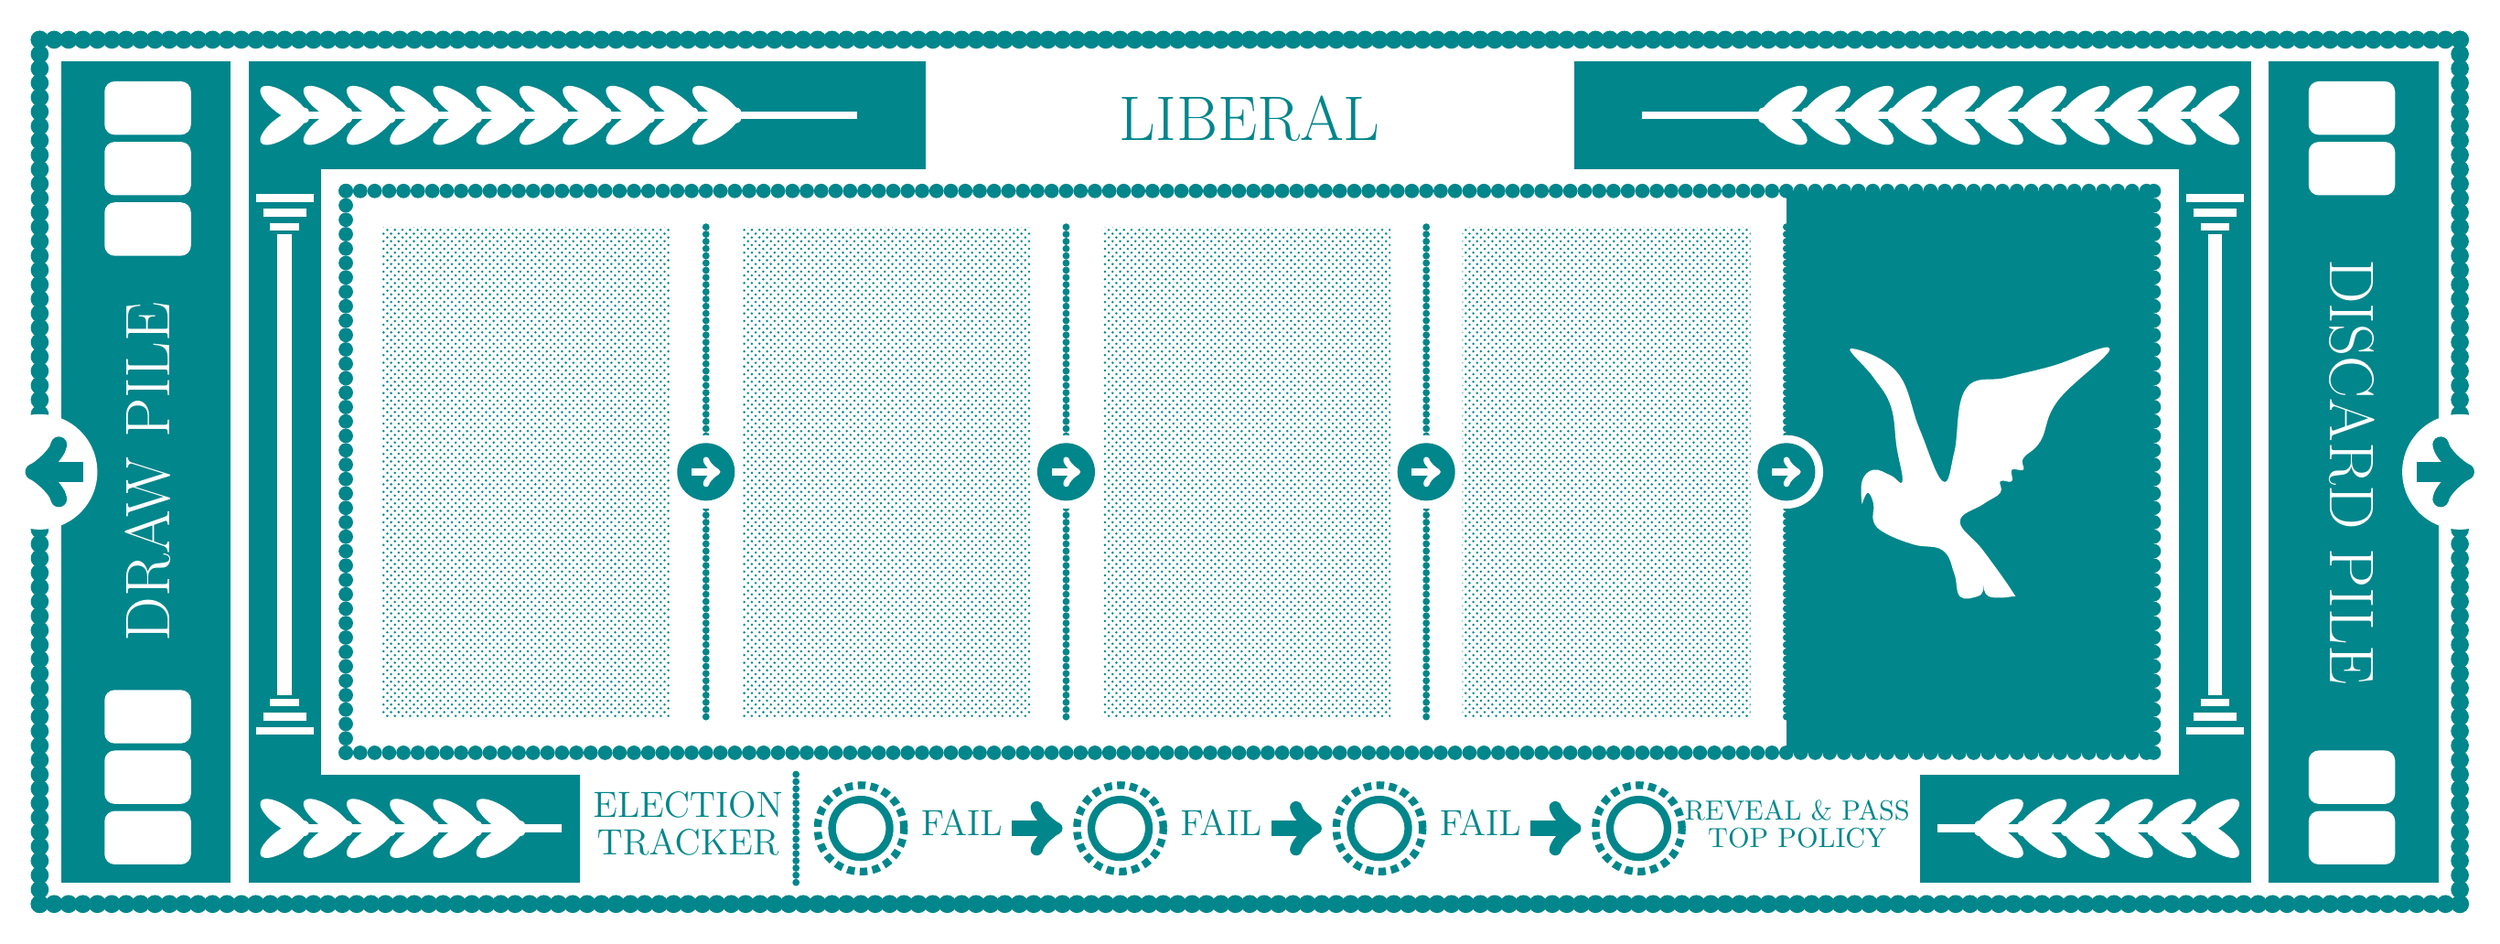
\begin{tikzpicture}		
		
		% Exterior clipping lines
		\clip (-0.2,-0.2) rectangle (33.8,12.2);
		
		% Exterior line of points
		\foreach \y in {0,0.2,...,12}
		{
			\fill [liberal] (0,\y) circle (1.25mm);
			\fill [liberal] (33.6,\y) circle (1.25mm);
		}
		
		\foreach \x in {0, 0.2, ..., 33.6}
		{
			\fill [liberal] (\x,0) circle (1.25mm);
			\fill [liberal] (\x,12) circle (1.25mm);
		}
	
		% Lateral blue rectangles
		\fill [liberal] (0.3,0.3) rectangle (2.65,11.7);
		\fill [liberal] (30.95,0.3) rectangle (33.3,11.7);
		
		% Interior line of points
		\foreach \y in {2.1,2.3,...,9.9}
		{
			\fill [liberal] (4.25,\y) circle (1mm);
			\fill [liberal] (29.35,\y) circle (1mm);
		}
		
		\foreach \x in {4.25, 4.45, ..., 29.35}
		{
			\fill [liberal] (\x,2.1) circle (1mm);
			\fill [liberal] (\x,9.9) circle (1mm);
		}
	
		% Central-upper text
		\node at (16.8,10.9) [liberal] {\fontsize{60}{60}\selectfont LIBERAL};
		
		% Lines of points to separate policies
		\foreach \y in {2.6,2.7,...,9.4}
		{
			\fill [liberal] (9.25,\y) circle (0.5mm);
			\fill [liberal] (14.25,\y) circle (0.5mm);
			\fill [liberal] (19.25,\y) circle (0.5mm);
			\fill [liberal] (24.25,\y) circle (0.5mm);
		}
	
		% Dotted pattern for policies
		\fill [pattern=crosshatch dots, pattern color=liberal] (4.75,2.6) rectangle(8.75,9.4);
		\fill [pattern color=liberal, pattern=crosshatch dots] (9.75,2.6) rectangle(13.75,9.4);
		\fill [pattern color=liberal, pattern=crosshatch dots] (14.75,2.6) rectangle(18.75,9.4);
		\fill [pattern color=liberal, pattern=crosshatch dots] (19.75,2.6) rectangle(23.75,9.4);
		\fill [liberal] (24.25,2.1) rectangle (29.35, 9.9);
	
		% Arrows between policies
		\fill [white] (9.25,6) circle (5.1mm);
		\fill [liberal] (9.25,6) circle (4mm);
		\draw [line width= 3, white,->] (9.05,6)--(9.45,6);
		\fill [white] (14.25,6) circle (5.1mm);
		\fill [liberal] (14.25,6) circle (4mm);
		\draw [line width= 3, white,->] (14.05,6)--(14.45,6);
		\fill [white] (19.25,6) circle (5.1mm);
		\fill [liberal] (19.25,6) circle (4mm);
		\draw [line width= 3, white,->] (19.05,6)--(19.45,6);
		\fill [white] (24.25,6) circle (5.1mm);
		\fill [liberal] (24.25,6) circle (4mm);
		\draw [line width= 3, white,->] (24.05,6)--(24.45,6);
		
		% Liberal logo on last policy
		\begin{scope} [xshift=26.9cm,yshift=4.75cm,scale=0.4]
			\fill [white] plot[smooth, tension=.7] coordinates {(-4,2) (-4,2.8) (-3.6,3.2) (-3,3) (-2.6,2.8) (-2.8,4) (-3,5.4) (-3.6,6.4) (-4.4,7.4) (-2.8,6.6) (-2,4.6) (-1.2,2.8) (-0.8,3.8) (-0.4,6) (1,6.4) (2.6,6.8) (4.6,7.4) (2.8,5.6) (2.2,4.2) (1.6,3.6) (1.6,3.2) (1.2,3.2) (1.2,2.8) (0.8,2.8) (0.8,2.4) (0.2,2) (-0.6,1.4) (0.2,0.4) (1.2,-1) (1.2,-1.2) (0.4,-1.2) (0.2,-0.8) (0.2,-1) (0,-1.2) (-0.6,-1.2) (-0.8,-0.4) (-1.2,0.4) (-2.2,0.6) (-3.2,1) (-3.6,1.4) (-3.6,2) (-3.8,2.4) (-4,2)};
		\end{scope}
	
		% Blue rectangles next to text
		\fill[liberal] (2.9, 11.7) rectangle(12.3,10.2);
		\fill[liberal] (30.7, 11.7) rectangle(21.3,10.2);
		
		% White leaves on blue rectangles next to text
		\draw [white, line width=3] (22.25,10.95)--(30.25,10.95);
		\foreach \x in {24.2, 24.8, ..., 30.5}
		{
			\begin{scope}[xshift=\x cm, yshift=11.1cm,rotate=35]
				\fill [white] (0,0) ellipse (0.4 and 0.15);
			\end{scope}	
			\begin{scope}[xshift=\x cm, yshift=10.8cm,rotate=-35]
				\fill [white] (0,0) ellipse (0.4 and 0.15);
			\end{scope}	
		}
	
		\draw [white, line width=3] (3.35,10.95)--(11.35,10.95);
		\foreach \x in {3.4, 4, ..., 9.5}
		{
			\begin{scope}[xshift=\x cm, yshift=11.1cm,rotate=145]
				\fill [white] (0,0) ellipse (0.4 and 0.15);
			\end{scope}	
			\begin{scope}[xshift=\x cm, yshift=10.8cm,rotate=-145]
				\fill [white] (0,0) ellipse (0.4 and 0.15);
			\end{scope}	
		}

		% Decoration columns on side of central policy area
		\fill [liberal] (2.9, 10.2) rectangle(3.9, 1.8);
		\draw [white, line width=3] (3,2.4)--(3.8,2.4);
		\draw [white, line width=3] (3.1,2.6)--(3.7,2.6);
		\draw [white, line width=3] (3.2,2.8)--(3.6,2.8);		
		\draw [white, line width=3] (3,9.8)--(3.8,9.8);
		\draw [white, line width=3] (3.1,9.6)--(3.7,9.6);
		\draw [white, line width=3] (3.2,9.4)--(3.6,9.4);
		\fill [white] (3.3,9.3) rectangle(3.5,2.9);
		
		\fill [liberal] (29.7, 10.2) rectangle(30.7, 1.8);
		\draw [white, line width=3] (29.8,2.4)--(30.6,2.4);
		\draw [white, line width=3] (29.9,2.6)--(30.5,2.6);
		\draw [white, line width=3] (30,2.8)--(30.4,2.8);		
		\draw [white, line width=3] (29.8,9.8)--(30.6,9.8);
		\draw [white, line width=3] (29.9,9.6)--(30.5,9.6);
		\draw [white, line width=3] (30,9.4)--(30.4,9.4);
		\fill [white] (30.1,9.3) rectangle(30.3,2.9);
		
		% White leaves and blue rectangles on the lower side of board.
		\fill [liberal] (2.9, 0.3) rectangle (7.5,1.8);
		\draw [white, line width=3] (3.35,1.05)--(7.25,1.05);
		\foreach \x in {3.4, 4, ..., 7}
		{
			\begin{scope}[xshift=\x cm, yshift=1.2cm,rotate=145]
				\fill [white] (0,0) ellipse (0.4 and 0.15);
			\end{scope}	
			\begin{scope}[xshift=\x cm, yshift=0.9cm,rotate=-145]
				\fill [white] (0,0) ellipse (0.4 and 0.15);
			\end{scope}	
		}		
	
		\fill [liberal] (26.1, 0.3) rectangle (30.7,1.8);
		\draw [white, line width=3] (26.35,1.05)--(30.25,1.05);
		\foreach \x in {27.2, 27.8, ..., 30.5}
		{
			\begin{scope}[xshift=\x cm, yshift=1.2cm,rotate=35]
				\fill [white] (0,0) ellipse (0.4 and 0.15);
			\end{scope}	
			\begin{scope}[xshift=\x cm, yshift=0.9cm,rotate=-35]
				\fill [white] (0,0) ellipse (0.4 and 0.15);
			\end{scope}	
		}
		
		% Discard and draw piles
		\begin{scope}[xshift=1.5cm, yshift=9cm, scale=1.2]
			\foreach \y in {0, 0.7, 1.4}
			\fill [white, rounded corners] (-0.5,\y) rectangle (0.5,\y+0.618);
		\end{scope}
		\begin{scope}[xshift=1.5cm, yshift=0.55cm, scale=1.2]
			\foreach \y in {0, 0.7, 1.4}
			\fill [white, rounded corners] (-0.5,\y) rectangle (0.5,\y+0.618);
		\end{scope}
		\node at (1.5, 6) [white, rotate=90] {\fontsize{25}{25}\selectfont DRAW PILE};
		\fill [white] (0,6) circle (8mm);
		\draw [line width= 8, liberal,->] (0.6,6)--(-0.2,6);
		
		\begin{scope}[xshift=32.1cm, yshift=9cm, scale=1.2]
			\foreach \y in {0.7, 1.4}
			\fill [white, rounded corners] (-0.5,\y) rectangle (0.5,\y+0.618);
		\end{scope}
		\begin{scope}[xshift=32.1cm, yshift=0.55cm, scale=1.2]
			\foreach \y in {0, 0.7}
			\fill [white, rounded corners] (-0.5,\y) rectangle (0.5,\y+0.618);
		\end{scope}
		\node at (32.1, 6) [white, rotate=-90] {\fontsize{25}{25}\selectfont DISCARD PILE};
		\fill [white] (33.6,6) circle (8mm);
		\draw [line width= 8, liberal,->] (33,6)--(33.8,6);
		
		% Election tracker
		\node at (9, 1.05) [liberal] {\fontsize{15}{15}\selectfont \begin{tabular}{c}
				ELECTION \\ TRACKER
		\end{tabular}};
		\foreach \y in {0.3,0.4,...,1.8}
		{
			\fill [liberal] (10.5,\y) circle (0.5mm);
		}
	
		\foreach \x in {11.4, 15, 18.6}
		{
			\begin{scope}[xshift=\x cm, yshift=1.05cm]
				\draw [liberal, line width=3]  (0,0) circle (4mm);
				\draw [liberal, line width=3, dotted]  (0,0) circle (6mm);
				\node at (1.4, 0) [liberal] {\fontsize{15}{15}\selectfont \begin{tabular}{c}
						FAIL
				\end{tabular}};
				\draw [line width = 6, liberal, ->] (2.1,0)--(2.8,0);
			\end{scope}
		}
		\begin{scope}[xshift=22.2 cm, yshift=1.05cm]
			\draw [liberal, line width=3]  (0,0) circle (4mm);
			\draw [liberal, line width=3, dotted]  (0,0) circle (6mm);
			\node at (2.2, 0) [liberal] {\fontsize{11}{11}\selectfont \begin{tabular}{c}
					REVEAL  \& PASS\\ TOP POLICY
			\end{tabular}};
		\end{scope}
		
	\end{tikzpicture}
\end{document}